\chapter{Theory} \label{CH:theory}

\section{Equations}\label{Sect:eqns}
Here is an example of an equation
\begin{equation}\label{eq:pyth}
  a^2+b^2=c^2,
\end{equation}
which states the square of the hypotenuse $c$ of a triangle is equal to the sum of the square of the other two sides ($a$ and $b$). 

A collection of similar equations can be written using the \verb|\align| environment, \eg, 
\begin{align}\label{eq:trig}
  \sin(\theta) &= \frac{1}{\csc(\theta)}\\
  \cos(\theta) &= \frac{1}{\sec(\theta)}\\
  \tan(\theta) &= \frac{1}{\cot(\theta)}
\end{align}

Cases can be added using
\begin{equation}
  x = \begin{cases}
    y, & \text{if $t = 1$;} \\
    z, & \text{otherwise.}
  \end{cases}
\end{equation}

\subsection{Symbols}\label{Sect:sym}
Symbols, like greek letters, can be used in equations, \eg, $\theta$, $\gamma$, and $\zeta$.  When variables are referenced in the text they should be written in mathmode and enclosed in dollar signs.  For example, $a$ and a, which are written in math and text modes, respectively.

\section{Figures}\label{Sect:figs}
Figures can easily be added to your latex document.  Graphs and figures should be designed to be printed in black and white and clearly display information.  Considering using vectorized graphics that will remain sharp even if viewed zoomed (try zooming on Fig~\ref{fig:plot}).  The text in your figure should be legible and preferably the same size as the text in the rest of your document.

\begin{figure}[htbp]
  \centering
  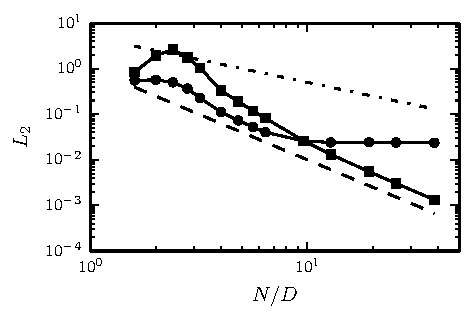
\includegraphics[width=0.6\textwidth]{figs/plot.pdf}
  \caption{This is a figure of some data.}
  \label{fig:plot}
\end{figure}

In \LaTeX{} figures may float and move around to a location that is optimized using mathematics. The htbp in the definition of the figure environment means here,top,bottom,page and is the order of preference for where the figure goes.  

Figure~\ref{fig:photo} shows you can also put pictures into \LaTeX{} documents.  The size of the figure is controlled by adjusting width.  If you find your figures are often floating to a page of their own consider changing their size and/or adding more text.

\begin{figure}[htbp]
  \centering
  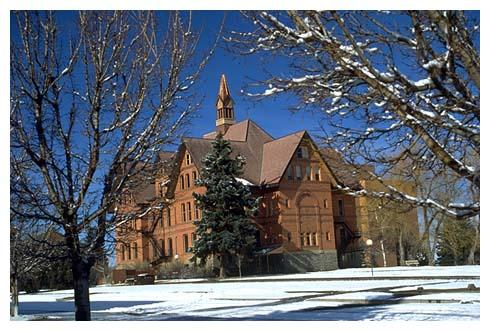
\includegraphics[width=0.6\textwidth]{figs/MSU.jpg}
  \caption{Montana Hall on Montana State University's campus.}
  \label{fig:photo}
\end{figure}

Figure~\ref{fig:tikz} shows that you can create figures directly within your \LaTeX{} document using, for example, the tikz package.
\begin{figure}[htbp]
  \centering
  % Define spring
  \tikzstyle{spring}=[thick,decorate,decoration={zigzag,pre length=0.75cm,post length=0.75cm,segment length=4}]
  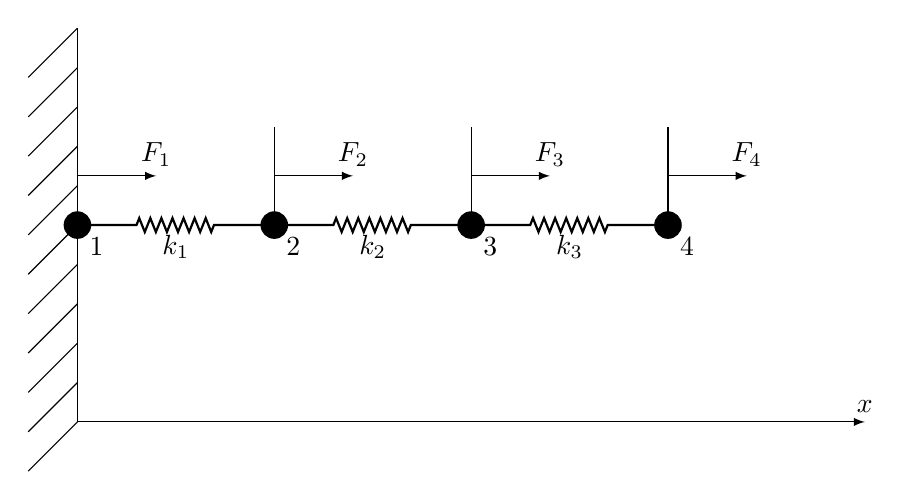
\begin{tikzpicture}[scale=2.5]
    % Draw wall
    \draw [] (1,0) -- (1,2);
    \foreach \y in {0,0.2,...,2.1}{
      \draw [] (1,\y) -- ++(-0.25,-0.25);
    }
    % Draw springs
    \foreach \x in {1,...,3} {
      \draw [spring] (\x,1) -- node[pos=0.5,below]{$k_{\x}$} (\x+1,1);
    }
    % Draw nodes and labels
    \foreach \x in {1,...,4} {
      \fill (\x,1) circle (0.07cm);
      \node [below right=0.03cm] at (\x,1) {$\x$};
      \draw (\x,1) -- (\x,1.5);
      \draw [arrows=-latex] (\x,1.25) -- node[pos=1,above]{$F_{\x}$} (\x+0.4,1.25);
    }
    % Draw axis
    \draw [arrows=-latex] (1,0) -- node[pos=1,above]{$x$}(5,0);
  \end{tikzpicture}
  \caption{Figure created using the tikz package.}
  \label{fig:tikz}
\end{figure}

\begin{figure}[P!]
  \centering
  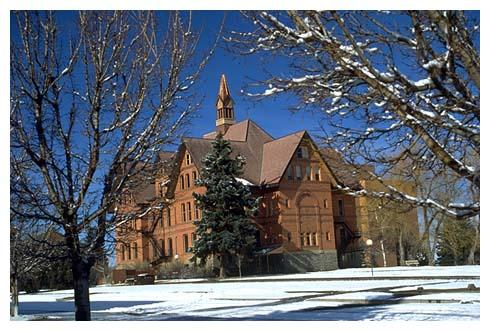
\includegraphics[width=0.6\textwidth]{figs/MSU.jpg}
  \caption{Figure forced to be on page by itself.}
  \label{fig:page}
\end{figure}

\clearpage

\section{Tables}\label{Sect:tabs}
Tables can be created directly in your \LaTeX{} document.  Table~\ref{tab:ice} shows how a short caption can be used in the table of contents and a long caption in the figure.  In the table of contents ``Area of ice sheet'' is listed and above the table ``Area of ice sheet in millions of square miles with time.'' is shown.  This is done by adding an optional argument to the \verb|\caption| command, \ie, \verb|\caption[Short Caption]{Long Caption}|.

\begin{table}[htbp]
  \centering
  \caption[Area of ice sheet]{Area of ice sheet in millions of square miles with time.}
  \label{tab:ice}
  \begin{tabular}{c | ccccccc}
    Year  & 1985 & 1990 & 1995 & 2000 & 2005 & 2010 & 2015\\\hline
    Area  & 16.2 & 15.5   & 15.2  & 15.5  & 14.6 & 15.4 & 14.5 
  \end{tabular}
\end{table}

\section{Algorithms}\label{Sect:Alg}
Algorithms can be added using the algorithmic environment as shown in Algorithm~\ref{alg:example}.
\begin{algorithm}[htbp]
%\textbf{Algorithm} Compete
\begin{algorithmic}[1]
\STATE \textbf{Input:} Function $f$ to optimize, subpopulations $\mathcal{S}$
\STATE \textbf{Output:} Full global solution $\boldsymbol{G}$
\STATE \hspace{0pt}{\textbf{//} Iterate over random permutation of $\boldsymbol{X}$}
\STATE \hspace{0pt}{\textbf{for each }{{$ X_i \in \boldsymbol{X}$} \textbf{do}}} \label{opa_compete:loop:1}
\STATE \hspace{8pt}{\textbf{//} Initialize comparison variables}
\STATE \hspace{8pt}{$bestFit \leftarrow \infty$} \label{opa_compete:init:1}
\STATE \hspace{8pt}{$bestVal \leftarrow \boldsymbol{S}_{0}[X_i]$} \label{opa_compete:init:2}
\STATE \hspace{8pt}{\textbf{//} Iterate over random permutation of $\boldsymbol{S}$}
\STATE \hspace{8pt}{\textbf{for each }{$\boldsymbol{S}_j \in \mathcal{S} \textbf{ where } X_i \in \boldsymbol{S}_j$} \textbf{do}}
\STATE \hspace{16pt}{\textbf{//} Substitute subpopulation component into full global solution}
\STATE \hspace{16pt}{$G_i \leftarrow \boldsymbol{S}_{j}[X_i]$} \label{opa_compete:compare:1}
\STATE \hspace{16pt}{\textbf{//} Compare Fitness}
\STATE \hspace{16pt}{\textbf{if} $f(\boldsymbol{G}) \text{ is better than } bestFit $ \textbf{then}}
\STATE \hspace{24pt}$bestVal \leftarrow \boldsymbol{S}_j[X_i]$
\STATE \hspace{24pt}$bestFit \leftarrow f(\boldsymbol{G})$
\STATE \hspace{16pt}\textbf{endif}
\STATE \hspace{8pt}\textbf{endfor} \label{opa_compete:compare:2}
\STATE \hspace{8pt}{\textbf{//} Copy $bestVal$ into full global solution}
\STATE \hspace{8pt}$G_i \leftarrow bestVal$
\STATE \textbf{endfor}
\RETURN
\end{algorithmic}
\caption{Algorithm example}
\label{alg:example}
\end{algorithm} 

\section{References and Citations}\label{Sect:ref_cite}

\subsection{Referencing Other Parts of the Document}\label{Sect:ref}
Equations, figures, tables, sections, and chapters can be references using the \verb|\ref{label}| command.  For example, \verb|\ref{fig:plot}| references Fig.~\ref{fig:plot}.  

You can also use the \verb|\vref| command to also get the page number.  For example, \verb|\vref{fig:plot}| references Fig.~\vref{fig:plot}.

The \verb|label| used in the \verb|\ref| command can be anything you want to use. It is helpful to use a convention.  For example, all figures could have a label that starts with \verb|fig:| and all table labels could start with \verb|tab:|.

\subsection{Citing Others Work}\label{Sect:cite}
Citing others work is an important aspect of all scientific writing.  All citations should be placed in the .bib file(s) listed in your main.tex document.  Cite others work using the \verb|\cite| command, \eg,~\cite{owkes_mesh-decoupled_2015}.  Multiple citations should be done within one cite command, \eg,~\cite{desjardins_direct_2013,owkes_discontinuous_2013,owkes_computational_2014}.  
